%Punchline!

%make plot of delta [C/N] versus R0(1D), color code observed binned points by mass of the star

Given the measured amounts of mixing described in Section \ref{sec:obs} and the reduced density ratios computed for stars of various masses and metallicities described in Section \ref{sec:mesa_results}, it is now possible to compare the observed amounts of extra mixing to the predictions of various thermohaline models from Section \ref{sec:formalism}, and determine if the observed mixing is at least qualitatively consistent with the expectations of the thermohaline instability. We show in Figure \ref{Fig:punchline}

note that the scatter is also important here- if the mixing actually depends on B field, and that depends randomly on the star (or on the stellar M/Z combo on average), then stars of the same R0 should have a range of mixi-ness. If R0 is the only parameter that matters, then mixing should strongly correlate with R0 with only minimal/ observational measurement scatter. 

%FIGURE solar---------------------------------------------------
\begin{figure*}[!htb]
\begin{minipage}{1.0\textwidth}
\begin{center}

\def\stackalignment{l}
\subfigure{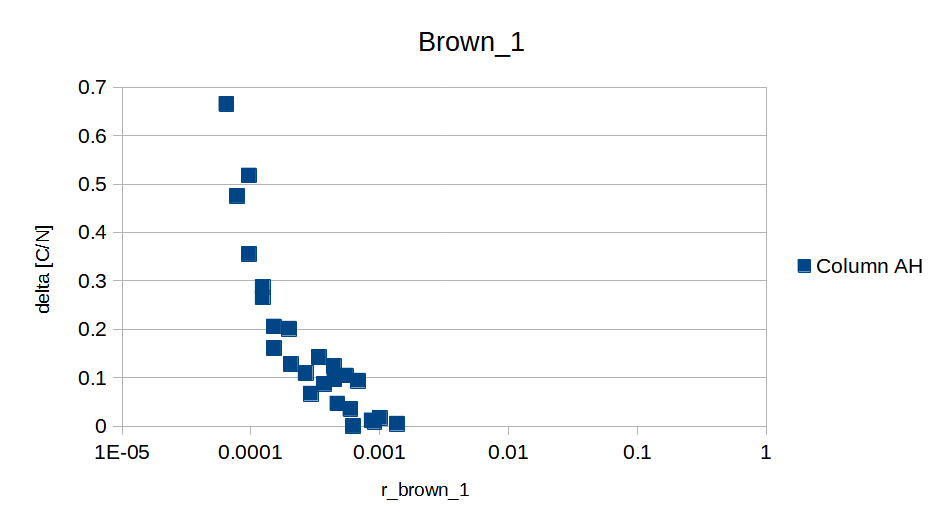
\includegraphics[width=0.43\textwidth,clip=true, trim=0.5in 0in 2.1in 0.3in]{figures/brown_1_log.png}}
\subfigure{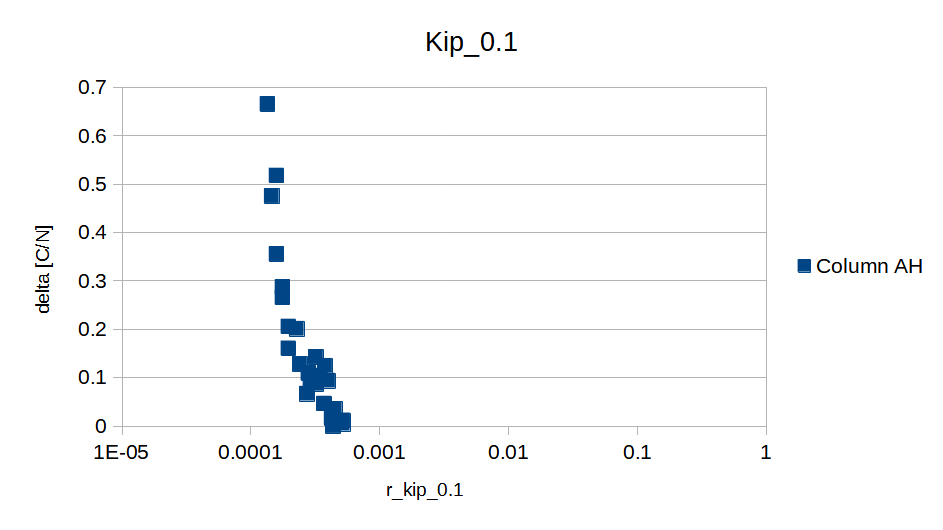
\includegraphics[width=0.43\textwidth,clip=true, trim=0.5in 0in 2.1in 0.3in]{figures/kip_0.1_log.png}}

\subfigure{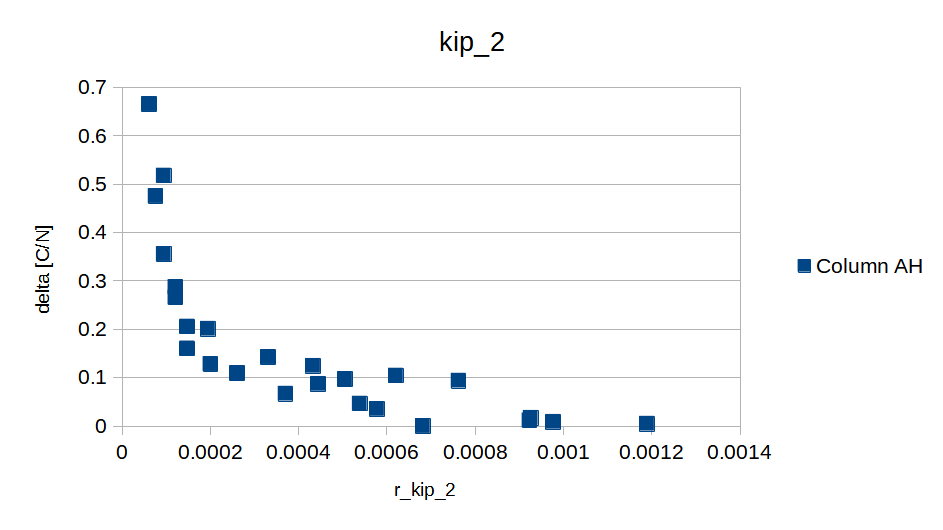
\includegraphics[width=0.43\textwidth,clip=true, trim=0.5in 0in 2.1in 0.3in]{figures/kip_2.png}}
\subfigure{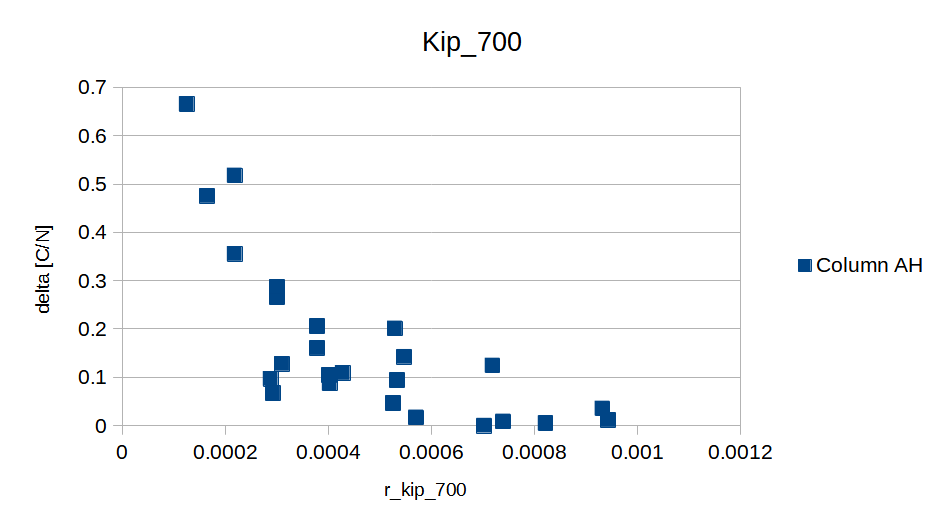
\includegraphics[width=0.43\textwidth,clip=true, trim=0.5in 0in 2.1in 0.3in]{figures/kip_700.png}}

\caption{Corrected measurements of the change in [C/N] near the red giant branch bump, compared to the reduced density ratio inferred from one-dimensional models using various thermohaline mixing prescriptions (Brown, Kippenhahn $\alpha=0.1$, Kippenhahn $\alpha=0.2$,Kippenhahn $\alpha=0.700$), color coded by the metallicity bin of each data point. In general there is a clear correlation between these parameters, suggesting that the observed mixing is related to fluid instabilities. More mixing is observed when the fluid is more unstable to the thermohaline instability, consistent with standard theories of thermohaline mixing, and observations do not probe high values of the reduced density ratios where magnetic fields may be important. }
\label{Fig:punchline}
\end{center}
\end{minipage}
\end{figure*}
